The following three types of image filters have been designed:
\begin{itemize}
\item Red-Filter
\item Green-Filter
\item Blue-Filter
\end{itemize}
These simple filters generates data, that just includes the \gls{rgb} values of a 32-Bit \gls{rgb} data set, regarding to the chosen logic of the dynamic partial reconfiguration application. Figure \ref{fig:imagefilter} describes the principle of the filter functionality. The logic of these filters is connected to the AXI-Lite Bus with the same Wrapper-Interface and is addressable by a common Linux-Device-Driver.\\
\begin{figure}[h]
\centering
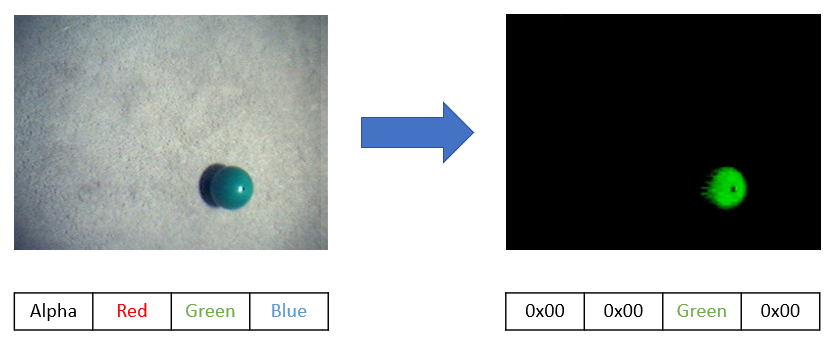
\includegraphics[width=1\textwidth]{sections/methodology/ImageFilter.PNG}
\caption{\label{fig:imagefilter} Green Filter example}
\end{figure}
The different cores are added to the system design via the concept described in section \ref{sssec:partialreconfigurationsetup} at the address $0x7E430000$ with the size of $64K$.  The logic behind the common wrapper uses 2 software accesible registers, each 32-bit wide:\\
\begin{tabular}{ll}
	Address & Name \\
	base     & write\_reg\\
	base + 4 & read\_reg\\
\end{tabular}\\
Value of the write_register is processed to the synthesized filter logic instance and then written to the read_register. The related linux device driver \ref{sssec:linuxkernelmodules} iterates the raw \gls{rgb} data each value after each other, during a write process to the device driver, and stores the filtered data, for reading from the device driver.